\label{par:lien_rock_equiv}
Pour comprendre les résultats de convergence précédents (\ref{par:etude_diff_rock4}), le profil des erreurs a été tracé (voir \ref{fig:error_profiles_landscape}) pour chaque méthode numérique et pour différents régimes de CFL ; puis 
ces observations ont été reliées aux équations équivalentes développées en \ref{par:contrib_2}. 
Cette mise en relation est cohérente car les équations équivalentes ont été calculées pour un schéma d'intégration en temps ERK2 et l'expérience a été réalisée avec 
ROCK2 qui est une ERK2 stabilisée.\\
Les résultats précédents sont confirmés:
\begin{enumerate}
    \item Pour les petites CFL, les méthodes avec reconstruction sont moins précisés que les méthodes sans reconstruction.
    \item Il existe une gamme de CFL très précise pour laquelle les schémas avec reconstruction sur-performent les autres méthodes.
\end{enumerate}
Munis de ces nouveaux résultats, une première hypothèse est formulée puis invalidée, avant qu'une seconde ne soit proposée et validée.
\subsubsection{Première Hypothèse}
\textbf{L'observation} suivante a de plus été faite: \textit{il semble que le profil de l'erreur avec reconstruction ressemble à la dérivée spatiale d'ordre quatre
de la solution et que le signe de cette erreur change avec la CFL}.\\
\textbf{Une première hypothèse} a d'abord été proposée: \textit{l'évolution du profil d'erreur selon la CFL s'explique par le terme $\Delta x^{2}\, D \, \Bigl( 
        \frac{\lambda}{2} (2^{2 \Delta l} - 1) + \frac{2^{2 \Delta l} }{12} (1 - 3 \Delta l)
        \Bigr)\frac{\partial^{4}u}{\partial x^{4}}$ dans l'équation équivalente \eqref{eq:equiv_cfl_recons}.}
En effet pour les grandes CFL le coefficient $\frac{\lambda}{2} (2^{2 \Delta l} - 1) + \frac{2^{2 \Delta l} }{12} (1 - 3 \Delta l)$ est positif et pour les petites CFL il est négatif, pour $\lambda = \frac{4^{\Delta l}}{6}\,\frac{3 \Delta l - 1 }{4^{\Delta l}-1} \underbrace{>}_{\Delta l >0} 0$ ce coefficient serait null expliquant 
chute de l'erreur pour ces CFL, l'erreur s'allégeant du terme d'ordre deux.\\
\textbf{Validation expérimentale:} Pour valider cette hypothèse, une régression linéaire entre l'erreur numérique et la dérivée $4^e$ de la solution a été réalisée par 
une méthode des moindres carrées : $$\min_{\alpha \in \mathbb R} \Vert \alpha \partial_x^4 u - \text{err} \Vert^2.$$
Ce modèle (fig. \ref{fig:derive4_vs_err}) explique bien l'erreur pour les petites CFL ($R^2>0.9$) mais mal pour les grandes CFL ($R^2 \sim 0.2$).
\begin{figure}[htpb]
    \centering
    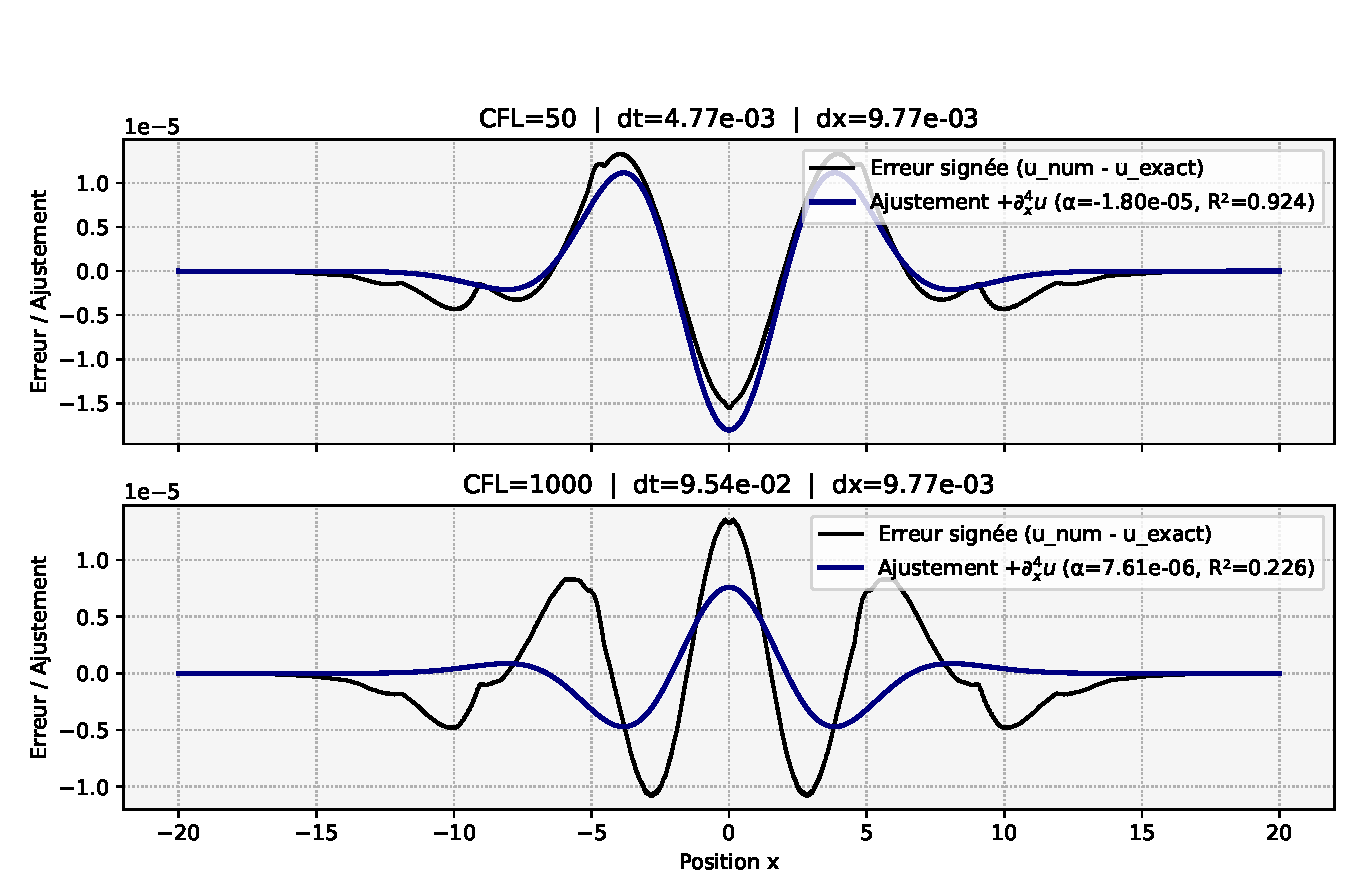
\includegraphics[width=0.75\textwidth]{media/4_travail/3/erreur_vs_deriv4.pdf}
    \caption{Régression entre l'erreur numérique expérimentale (AMR + reconstruction fine) et la dérivées $4^e$ de la solution.}
    \label{fig:derive4_vs_err}
\end{figure}
\newpage
\subsubsection{Seconde Hypothèse}
\textbf{Une seconde observation} a alors révisé la première: \textit{à grande CFL, l'erreur ne ressemble pas à l'opposé de $\partial_x^4 u$ mais à 
$\partial_x^6 u$.}\\
\textbf{Une seconde hypothèse} a alors été émise :
    \begin{itemize}
        \item[$\diamond$] Pour les grandes CFL, le terme $- \Delta x^4 \frac{D}{6} \lambda^2 \partial_x^6 u$, quadratique en $\lambda$ domine dans \eqref{eq:equiv_cfl_recons},
        \item[$\diamond$] Pour les petites CFL, le terme $\Delta x^{2}\, D \, \Bigl(\frac{\lambda}{2} (2^{2 \Delta l} - 1) + \frac{2^{2 \Delta l} }{12} (1 - 3 \Delta l)\Bigr)\frac{\partial^{4}u}{\partial x^{4}}$, affine en $\lambda$ domine.
    \end{itemize}
    Le fait que pour les petites CFL le schéma \texttt{II} (sans reconstruction) soit plus précis que le schéma \texttt{III} (avec reconstruction),
    s'explique simplement par le fait que la constante d'erreur pondérant terme d'erreur dominant $\Delta x^2 \partial_x^4 u$ est plus grand pour le schéma \texttt{III}:
\begin{center}
    \renewcommand{\arraystretch}{1}
    \begin{tabular}{@{}clc@{}}
        \toprule
        \textbf{Schéma n\textsuperscript{o}} & \textbf{Évaluation des flux} &
        \makecell[c]{\textbf{Constante pondérant l'erreur en $\Delta x^{2}\,\partial_{x}^{4}u$}\\
                    \textbf{(dominante quand $\lambda$ est petite)}} \\
        \midrule
        I   & $\varnothing$ AMR          & $\dfrac{D}{12}$ \\[1mm]
        II  & Sans reconstruction         & $2^{\Delta l}\,\dfrac{D}{12}$ \\[1mm]
        III & Avec reconstruction         &
            $D\,\Bigl(\dfrac{\lambda}{2}\,(2^{2\Delta l}-1)
            + \dfrac{2^{2\Delta l}}{12}\,(1-3\Delta l)\Bigr)$ \\[1mm]
        \bottomrule
    \end{tabular}
\end{center}
\textbf{Validation expérimentale: } pour valider empiriquement cette nouvelle hypothèse, l'erreurs a été modélisée par moindre carré comme $\text{err} \approx \alpha \partial_x^4 u + \beta \partial_x^6u$. 
Ce modèle explique très bien l'erreur pour tous les régimes de CFL (voir \ref{fig:derivees_vs_err}).
\begin{figure}[h!]
    \centering
    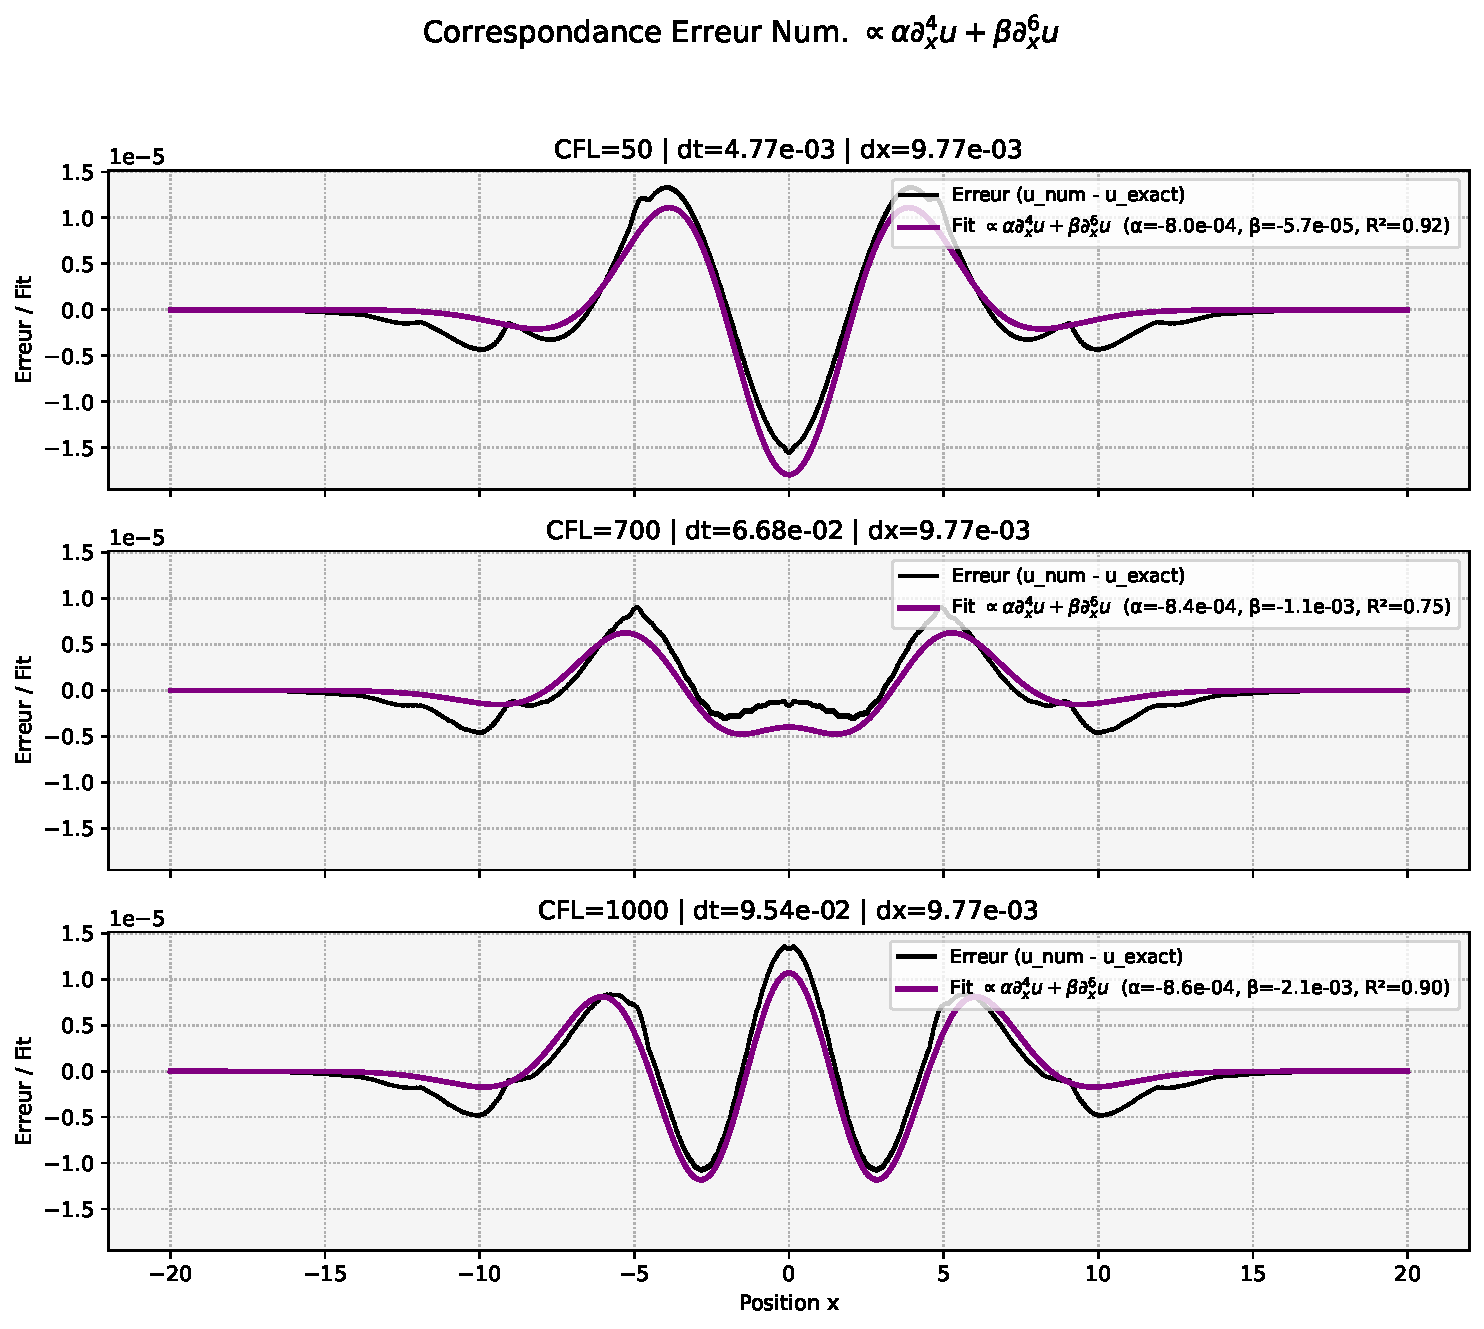
\includegraphics[width=0.75\textwidth]{media/4_travail/3/derivees_spatiales_VS_err_num.pdf}
    \caption{Régression entre l'erreur numérique expérimentale (AMR + reconstruction fine) et une combinaison linéaire des dérivées $4^e$ et $6^e$ de la solution.}
    \label{fig:derivees_vs_err}
\end{figure}\\
\textbf{Remarque:} la plage de CFL où la méthode avec reconstruction est plus la précise correspond en fait au cas ou les profils de $ \alpha \partial_x^4 u$
de $\beta \partial_x^6 u$ se compensent. C'est donc un comportement tout à fait accidentel lié au fait que les dérives de la courbe de Gauss sont en quelque sort "en opposition de phase".\\
\textbf{Analyse retrospective:} Le comportement observé s'explique par une \emph{incohérence précision} entre le schéma et la reconstruction.
Une prédiction à trois points n'apporte pas d'information supplémentaire par rapport au schéma spatial d'ordre deux :
elle reste du même ordre de précision et ne réduit donc pas le terme d'erreur dominant.
Dans ces conditions, la reconstruction ajoute du bruit au lieu d'améliorer la solution.\\
\textbf{Complément important:} Ce n'est pas présenté ici, mais le travail à été refait avec un prédicteur à 5 points, permettant d'approximer correctement la dérivée d'ordre quatre.
Alors la reconstruction apporte un gain notable, les solutions numériques avec et sans MRA sont dans ce cas très proches.